% Options for packages loaded elsewhere
\PassOptionsToPackage{unicode}{hyperref}
\PassOptionsToPackage{hyphens}{url}
\documentclass[
]{article}
\usepackage{xcolor}
\usepackage{amsmath,amssymb}
\setcounter{secnumdepth}{-\maxdimen} % remove section numbering
\usepackage{iftex}
\ifPDFTeX
  \usepackage[T1]{fontenc}
  \usepackage[utf8]{inputenc}
  \usepackage{textcomp} % provide euro and other symbols
\else % if luatex or xetex
  \usepackage{unicode-math} % this also loads fontspec
  \defaultfontfeatures{Scale=MatchLowercase}
  \defaultfontfeatures[\rmfamily]{Ligatures=TeX,Scale=1}
\fi
\usepackage{lmodern}
\ifPDFTeX\else
  % xetex/luatex font selection
\fi
% Use upquote if available, for straight quotes in verbatim environments
\IfFileExists{upquote.sty}{\usepackage{upquote}}{}
\IfFileExists{microtype.sty}{% use microtype if available
  \usepackage[]{microtype}
  \UseMicrotypeSet[protrusion]{basicmath} % disable protrusion for tt fonts
}{}
\makeatletter
\@ifundefined{KOMAClassName}{% if non-KOMA class
  \IfFileExists{parskip.sty}{%
    \usepackage{parskip}
  }{% else
    \setlength{\parindent}{0pt}
    \setlength{\parskip}{6pt plus 2pt minus 1pt}}
}{% if KOMA class
  \KOMAoptions{parskip=half}}
\makeatother
\usepackage{longtable,booktabs,array}
\newcounter{none} % for unnumbered tables
\usepackage{calc} % for calculating minipage widths
% Correct order of tables after \paragraph or \subparagraph
\usepackage{etoolbox}
\makeatletter
\patchcmd\longtable{\par}{\if@noskipsec\mbox{}\fi\par}{}{}
\makeatother
% Allow footnotes in longtable head/foot
\IfFileExists{footnotehyper.sty}{\usepackage{footnotehyper}}{\usepackage{footnote}}
\makesavenoteenv{longtable}
\usepackage{graphicx}
\makeatletter
\newsavebox\pandoc@box
\newcommand*\pandocbounded[1]{% scales image to fit in text height/width
  \sbox\pandoc@box{#1}%
  \Gscale@div\@tempa{\textheight}{\dimexpr\ht\pandoc@box+\dp\pandoc@box\relax}%
  \Gscale@div\@tempb{\linewidth}{\wd\pandoc@box}%
  \ifdim\@tempb\p@<\@tempa\p@\let\@tempa\@tempb\fi% select the smaller of both
  \ifdim\@tempa\p@<\p@\scalebox{\@tempa}{\usebox\pandoc@box}%
  \else\usebox{\pandoc@box}%
  \fi%
}
% Set default figure placement to htbp
\def\fps@figure{htbp}
\makeatother
\setlength{\emergencystretch}{3em} % prevent overfull lines
\providecommand{\tightlist}{%
  \setlength{\itemsep}{0pt}\setlength{\parskip}{0pt}}
\usepackage{bookmark}
\IfFileExists{xurl.sty}{\usepackage{xurl}}{} % add URL line breaks if available
\urlstyle{same}
\hypersetup{
  hidelinks,
  pdfcreator={LaTeX via pandoc}}

\author{}
\date{}

\begin{document}

\section{Conserved Quantities and Uncertainty as Phase-Space Area --- A
Unified Viewpoint of Symplectic Symmetry, Wick Rotation, and Stone's
Theorem}\label{conserved-quantities-and-uncertainty-as-phase-space-area-a-unified-viewpoint-of-symplectic-symmetry-wick-rotation-and-stones-theorem}

\textbf{Author}: Noriaki Kihara \textbf{Affiliation}: WF System Co.,
Ltd.~/ Faculty of Engineering Science, Osaka University (graduate)
\textbf{ORCID}:
\href{https://orcid.org/0009-0004-6753-4020}{0009-0004-6753-4020}
\textbf{Version}: v10 \textbf{Date}: June 2026 \textbf{License}: CC BY
4.0

\begin{center}\rule{0.5\linewidth}{0.5pt}\end{center}

\subsection{Character of This Note}\label{character-of-this-note}

\textbf{This is an observation paper. It does not propose a new physical
theory.}

This note does not modify standard quantum theory. It does not reject
Wick rotation. It does not declare the Minkowski metric erroneous. It
changes no observable prediction. Its entire claim is to
\textbf{re-arrange and observe, from the single viewpoint of phase-space
area}, structures that already exist within standard mathematics --- the
Heisenberg--Gabor uncertainty relation, Robertson's inequality, the
symplectic symmetry \(\mathrm{Sp}(2,\mathbb{R})\cong\mathrm{SU}(1,1)\),
Stone's theorem, and Wick rotation.

We emphasize: what this note does is to confirm that the \(i\) appearing
in Wick rotation and the \(i\) of the skew-adjoint generator in Stone's
theorem are described by \textbf{the same complex structure} of the
standard complex Hilbert space, and to re-read this formal
correspondence from the viewpoint of phase-space area (this is not a
replacement). Consequently, the invariance of the speed of light and the
causal (light-cone) order are \textbf{inherited} unchanged from standard
theory. What this note adds to standard theory is not a new numerical
prediction, but only a unified re-reading of known structures from one
viewpoint.

This note does \textbf{not} claim any of the following:

\begin{itemize}
\tightlist
\item
  Modification of the mathematical predictions of standard quantum
  theory or special relativity
\item
  Any assertion that Wick rotation or the Minkowski metric is ``wrong''
\item
  Derivation of the metric signature, the imaginary unit, or the complex
  structure
\item
  Derivation of new physical constants, cross sections, or decay rates
\item
  Proof of new mathematical theorems
\end{itemize}

Evaluation and interpretation are left to the reader.

\begin{center}\rule{0.5\linewidth}{0.5pt}\end{center}

\subsection{Abstract}\label{abstract}

Classical signal theory (Fourier analysis, sampling) and quantum theory
share a common currency when read as structures on the phase plane
\((q,p)\): the action \(\oint p\,dq\) (a conserved quantity) and the
area spanned by uncertainty (fluctuation) are both measured as the
symplectic area spanned by a conjugate pair. Taking this ``area as
common currency'' as the starting point, this note observes three known
facts from a single viewpoint.

First, the zero-point \(\tfrac12\) appearing in semiclassical
quantization \(\oint p\,dq=(n+\tfrac12)h\), the equality condition of
Robertson's inequality (the Gaussian ground state), the Maslov index
(boundary character), and the lowest-weight representation of
\(\mathrm{SU}(1,1)\) (Bargmann index) appear as three facets of the
common structure of half-integer weights of the metaplectic
representation, the double cover of \(\mathrm{Sp}(2,\mathbb{R})\) (the
three are not, however, numerically identical).

Second, the totality of area-preserving linear transformations forms
\(\mathrm{Sp}(2,\mathbb{R})\cong\mathrm{SU}(1,1)\); the symplectic area
is kept invariant by the group action (on the representation-theoretic
side, the Casimir corresponds as the representation label), and
squeezing, chirp, and phase rotation are group actions. In particular,
the non-compact subgroup (squeezing) is isomorphic to the Lorentz boost
on phase space, with velocity appearing as \(v/c=\tanh\eta\) and shape
parameter \(k=e^{2\eta}\).

Third, under the above symmetry (the stage of observation is throughout
an even-dimensional phase space \(\mathbb{R}^{2n}\) spanned by \(n\)
conjugate pairs), the hyperbolic structure and the imaginary unit \(i\)
appearing in Wick rotation and the Lorentz boost can be \textbf{re-read}
in the language of the representation form that Stone's theorem assigns
to the generator of continuous evolution (skew-adjoint \(=i\times\)
self-adjoint). This reading is observationally equivalent to Wick
rotation and to standard quantum theory (this note does not derive \(i\)
or the metric signature). From this viewpoint, whether a given
two-dimensional plane appears as a rotation (sign \(+\)) or a hyperbola
(sign \(-\)) is relative to whether one treats the one-parameter
subgroup acting on that plane as compact time evolution or as a
non-compact evolution corresponding to analytic continuation/boost, in
just the same way as the coordinate-dependence of the imaginary-time
direction in Wick rotation. Also, because of the uncertainty floor
\(\tfrac12\), there is no zero-area point-like state in phase space.

This note makes no new claim and is limited to a juxtaposed observation
of these known structures from one viewpoint.

\begin{center}\rule{0.5\linewidth}{0.5pt}\end{center}

\subsection{§1 Motivation: Area as Common
Currency}\label{motivation-area-as-common-currency}

\subsubsection{1.1 The rectangular wave and the divergence of
bandwidth}\label{the-rectangular-wave-and-the-divergence-of-bandwidth}

One of the most basic objects in signal theory is the rectangular pulse.
The Fourier transform of a single rectangle
\(g(t)=A\,\mathrm{rect}(t/\tau)\) of width \(\tau\) and height \(A\) is

\[G(\nu)=A\tau\,\mathrm{sinc}(\nu\tau),\qquad \mathrm{sinc}(x)\equiv\frac{\sin(\pi x)}{\pi x}\]

with a tail \(|G(\nu)|^2\sim 1/\nu^2\). Hence the mean-square bandwidth

\[\langle\nu^2\rangle\propto\int \nu^2|G(\nu)|^2\,d\nu\]

\textbf{diverges}. The time--bandwidth rms product of the rectangle is
infinite, and it \textbf{cannot attain} the minimum value (the
\(1/4\pi\) below) --- it does not fall short of it but exceeds it
without bound. As the price of perfectly sharp corners, the rectangle
cannot maintain a stationary profile in a dispersive continuum.
Incidentally, maximal energy concentration for finite time and finite
band is given not by the rectangle but by the prolate spheroidal wave
functions {[}21{]}, and the simultaneous concentration of \(g\) and
\(G\) is bounded by a Hardy-type limit {[}22{]}.

To obtain a finite rms bandwidth, one needs smoothing of corners,
band-limiting approximation, or an effective cutoff via discrete
sampling. The sampling theorem (Shannon 1949) {[}7{]} states that a
band-limited continuous signal can be reconstructed from discrete
samples; for a sample interval \(a\), the distinguishable frequencies
are limited to \(|\nu|\le\nu_s/2\) (the Nyquist edge, \(\lambda\ge 2a\)
in wavelength). This note refers to discrete sampling only as one
example of an effective cutoff.

\subsubsection{1.2 Two areas: count and
floor}\label{two-areas-count-and-floor}

The discussion of the rectangular pulse connects naturally to the theme
of this note, ``area.'' When the stage on which an observer reads
quantities is taken to be the phase plane of the conjugate pair
\((q,p)\), the meaningful invariants are concentrated in the dimension
of area (action):

\begin{itemize}
\tightlist
\item
  \(\oint p\,dq\): the area enclosed by a closed orbit (action, a
  conserved quantity).
\item
  the area of fluctuation (uncertainty): the symplectic area
  \(\sqrt{\det\Sigma}\) of a pure Gaussian state (which equals
  \(\Delta q\,\Delta p\) in a zero-correlation frame).
\end{itemize}

Both have the dimension of ``(a quantity along \(q\)) \(\times\) (a
quantity along \(p\))'' (action \(=\) phase-space area). It is area ---
not length or volume --- because \(q\) and \(p\) are a single conjugate
pair, and what a symplectic transformation preserves is area.

\textbf{However, the two share the same dimension but are not the same
number.} Since this distinction is used repeatedly here, we separate the
three quantities explicitly.

{\def\LTcaptype{none} % do not increment counter
\begin{longtable}[]{@{}
  >{\raggedright\arraybackslash}p{(\linewidth - 4\tabcolsep) * \real{0.3333}}
  >{\raggedright\arraybackslash}p{(\linewidth - 4\tabcolsep) * \real{0.3333}}
  >{\raggedright\arraybackslash}p{(\linewidth - 4\tabcolsep) * \real{0.3333}}@{}}
\toprule\noalign{}
\begin{minipage}[b]{\linewidth}\raggedright
Quantity
\end{minipage} & \begin{minipage}[b]{\linewidth}\raggedright
Value (in \(\hbar\))
\end{minipage} & \begin{minipage}[b]{\linewidth}\raggedright
Meaning
\end{minipage} \\
\midrule\noalign{}
\endhead
\bottomrule\noalign{}
\endlastfoot
Floor of the fluctuation area \(\sqrt{\det\Sigma}\) (=
\(\Delta q\,\Delta p\) in zero-correlation frame) & \(\hbar/2\) & Lower
bound satisfied by all states (Robertson) \\
Orbital action of the ground state \(\oint p\,dq\) &
\(\tfrac12 h=\pi\hbar\) & Semiclassical action of \(n=0\) \\
Phase-space cell per state & \(h=2\pi\hbar\) & Density of states
\(1/h\) \\
\end{longtable}
}

For the harmonic-oscillator state \(n\), the orbital action
\(\oint p\,dq=(n+\tfrac12)h\) grows with \(n\), whereas the fluctuation
area stays at \(\hbar/2\) independent of \(n\). The correct relation is

\[\oint p\,dq = n\,h + \tfrac12 h\qquad(\text{count}\times\text{cell }h\ +\ \text{the leftover }\tfrac12 h)\]

and \(\oint p\,dq\) is the total counting ``how many minimum-uncertainty
cells.'' \textbf{When this note speaks of ``area as common currency,''
it means that both \(\Delta q\,\Delta p\) and \(\oint p\,dq\) are
measured in the unit of the same symplectic area --- not that their
numerical values coincide.} The \(\hbar/2,\ \pi\hbar,\ 2\pi\hbar\) in
the table above differ by factors \(2\pi\) and \(4\pi\) and must not be
conflated. We adopt this distinction as a consistent viewpoint.

\begin{center}\rule{0.5\linewidth}{0.5pt}\end{center}

\subsection{\texorpdfstring{§2 Three Settings in Which the Zero-Point
\(\tfrac12\)
Appears}{§2 Three Settings in Which the Zero-Point \textbackslash tfrac12 Appears}}\label{three-settings-in-which-the-zero-point-tfrac12-appears}

\subsubsection{2.1 Semiclassical
quantization}\label{semiclassical-quantization}

When momentum is quantized in a closed space (perimeter \(L\)), the
phase area of one cycle is

\[\oint p\,dq = p_n L = \Big(\hbar\cdot\frac{2\pi n}{L}\Big)L = n\,h\]

so the conserved quantity is the number \(n\) of waves fitting in the
closed space times \(h\). In the semiclassical (WKB/EBK) approximation,
a fractional part determined by the boundary character is added:

\[\oint p\,dq = \Big(n+\frac{\mu}{4}\Big)h\]

(\(\mu\) is the Maslov index). For smooth confinement (harmonic), two
turning points each contribute \(\tfrac14\), so \(\mu=2\),
i.e.~fractional part \(\tfrac12\). For a hard wall (infinite well), the
idealization gives \(\oint p\,dq=n\,h\) (no \(+\tfrac12\)). But the
infinite well is the non-physical idealization of an infinite potential,
and real confinement is meaningful only as a limit of it. Note that even
in the infinite well each state satisfies the Robertson floor (for the
ground state
\(\Delta x\,\Delta p=\hbar\sqrt{(\pi^2-6)/12}\approx0.568\hbar>\hbar/2\)).
\textbf{That is, the uncertainty floor holds even in the infinite well,
whereas the action fractional part \(\tfrac12\) does not appear there.}
The two are independent quantities and must not be identified
numerically. Yet for the harmonic oscillator the two are both connected
to the metaplectic representation, and so appear in correspondence as a
half-integer structure (§2.4).

\subsubsection{2.2 Robertson's equality and the Gaussian ground
state}\label{robertsons-equality-and-the-gaussian-ground-state}

Inserting \(A=q,\ B=p,\ [q,p]=i\hbar\) into Robertson's inequality
(Robertson 1929) {[}2{]}

\[\Delta A\cdot\Delta B \ge \tfrac12\,\bigl|\langle[A,B]\rangle\bigr|\]

gives

\[\Delta q\cdot\Delta p \ge \frac{\hbar}{2}=\frac{h}{4\pi}.\]

This is the same theorem as the Gabor--Heisenberg inequality
\(\Delta t\cdot\Delta\nu\ge 1/4\pi\) of signal theory (Heisenberg 1927
{[}1{]}, Gabor 1946 {[}4{]}). Writing the equality condition

\[(A-\langle A\rangle)\,|\psi\rangle = i\lambda\,(B-\langle B\rangle)\,|\psi\rangle\quad(\lambda\in\mathbb{R})\]

in \(q,p\) gives a first-order differential equation whose solutions
are, up to translation, mean-momentum phase, width, and overall phase,
restricted to the Gaussian form \(\psi(q)\propto e^{-q^2/2\sigma^2}\).
These are the minimum-uncertainty states attaining the floor
\(\hbar/2\); measuring the representative (the harmonic-oscillator
ground state) by energy gives \(E_0=\tfrac12\hbar\omega\), and in
orbital action \(\oint p\,dq=\tfrac12 h\).

\textbf{Important remark (definition of ``area'' in this note)}: When a
chirp (shear) \(M_c=\begin{pmatrix}1&0\\\beta&1\end{pmatrix}\) is
applied later (§3), a correlation \(\mathrm{Cov}(q,p)\neq0\) is induced
between \(q,p\), and even for a pure Gaussian the simple marginal
product

\[\Delta q\,\Delta p=\frac{\hbar}{2}\sqrt{1+\beta^2}\ >\ \frac{\hbar}{2}\]

\textbf{increases}. That is, the marginal product \(\Delta q\,\Delta p\)
is not \(\mathrm{Sp}(2,\mathbb{R})\)-invariant, and saturates Robertson
only in a zero-correlation frame (a tilted ellipse saturates
Schrödinger--Robertson but not Robertson). What is genuinely invariant
under \(\mathrm{Sp}(2,\mathbb{R})\) is the square root of the
determinant of the covariance matrix \(\Sigma\), i.e.~the
\textbf{symplectic area} measured by the left side of the
Schrödinger--Robertson form

\[(\Delta q)^2(\Delta p)^2-\mathrm{Cov}(q,p)^2 \ge \frac{\hbar^2}{4}\]

(equal to \(\hbar/2\) for a pure Gaussian; the covariance-matrix
formulation is Simon--Sudarshan--Mukunda {[}23{]}). This is the
invariant captured by de Gosson's quantum blob {[}20{]}, and
\(\oint p\,dq\) is measured in this unit as well. \textbf{Hereafter,
whenever this note says ``area'' it consistently means this symplectic
area \(\sqrt{\det\Sigma}\), while the frame-dependent marginal product
\(\Delta q\,\Delta p\) is distinguished as the value in a
zero-correlation frame.}

\subsubsection{2.3 SU(1,1) lowest-weight
representation}\label{su11-lowest-weight-representation}

The Bargmann index characterizing the lowest-weight representation (the
representation starting from the ground state) of the symmetry group
\(\mathrm{SU}(1,1)\) discussed below is one of two values \(k=\tfrac14\)
or \(\tfrac34\), from which the fractional part of
\(\oint p\,dq=(n+\tfrac12)h\) is determined group-theoretically
(Bargmann 1947 {[}9{]}, Perelomov 1986 {[}10{]}).

\subsubsection{\texorpdfstring{2.4 Observation: the half-integer
structure running through the three
\(\tfrac12\)'s}{2.4 Observation: the half-integer structure running through the three \textbackslash tfrac12's}}\label{observation-the-half-integer-structure-running-through-the-three-tfrac12s}

The \(\tfrac12\)-type values appearing in the Maslov index (boundary
character), the Robertson floor (minimum-uncertainty state), and the
\(\mathrm{SU}(1,1)\) lowest weight (representation theory) are
\textbf{separate quantities arising from individually different
theorems} --- the value of the Maslov index itself depends on the system
and boundary conditions (as in §2.1, in the infinite well the
\(\tfrac12\) disappears), and the Robertson floor \(\hbar/2=h/4\pi\) is
a number of action dimension, differing even in dimension from the
dimensionless weights \(\tfrac14,\tfrac34\). Hence this note does not
regard the three as ``the same object.''

Yet that the three share a half-integer structure is not an unrelated
coincidence: \textbf{all of them can be understood as structures
connected to the metaplectic representation, the double cover, and the
half-integer phase.} Namely, the metaplectic representation (Weil
representation) {[}24{]} of the double cover
\(\mathrm{Mp}(2,\mathbb{R})\) (metaplectic group) of
\(\mathrm{Sp}(2,\mathbb{R})\) commonly underlies the three through its
half-integer weight. The ground state (lowest-weight state) saturating
the minimum symplectic area, the Maslov correction entering the
semiclassical action, and the Bargmann index appearing in the
\(\mathrm{SU}(1,1)\) lowest weight --- all of these connect to the
half-integer structure of this double cover.

Therefore this note neither over-identifies the three as ``the same
object arising from the same theorem'' nor regards them as ``three
unrelated coincidences.'' We read them as \textbf{a structure connected
to the half-integer weight of the metaplectic representation.} The §1.1
fact --- that the rectangle (fractional part \(0\)) cannot attain the
floor \(1/4\pi\) because of its rms bandwidth divergence, while the
Gaussian (fractional part \(\tfrac12\)) sits exactly at the floor --- is
also a facet of this structure. Semiclassical quantization
\(\oint p\,dq=(n+\tfrac12)h\) reads as ``the count \(n\) (an integer,
which mode) plus the unremovable leftover \(\tfrac12\) (the
uncertainty).''

\begin{center}\rule{0.5\linewidth}{0.5pt}\end{center}

\subsection{\texorpdfstring{§3 The Area-Preserving Symmetry Group
\(\mathrm{Sp}(2,\mathbb{R})\cong\mathrm{SU}(1,1)\)}{§3 The Area-Preserving Symmetry Group \textbackslash mathrm\{Sp\}(2,\textbackslash mathbb\{R\})\textbackslash cong\textbackslash mathrm\{SU\}(1,1)}}\label{the-area-preserving-symmetry-group-mathrmsp2mathbbrcongmathrmsu11}

\subsubsection{3.1 Area-preserving linear
transformations}\label{area-preserving-linear-transformations}

Taking the phase-plane vector to be \((q,p)\) and the symplectic form to
be \(J=\begin{pmatrix}0&1\\-1&0\end{pmatrix}\), an area-preserving
linear transformation \(M\) satisfies

\[M^{\mathsf T}JM=J\quad(\Longleftrightarrow\ \det M=1\ \text{in}\ 2\times2).\]

In \(2\times2\) the conditions \(M^{\mathsf T}JM=J\) and \(\det M=1\)
are equivalent, and
\(\mathrm{Sp}(2,\mathbb{R})=\mathrm{SL}(2,\mathbb{R})\). The following
three operations are elements of this group:

\begin{itemize}
\tightlist
\item
  Squeeze: \(M_s=\begin{pmatrix}e^{-r}&0\\0&e^{+r}\end{pmatrix}\)
  (compress one axis, stretch the other; area-invariant)
\item
  Rotation:
  \(M_\theta=\begin{pmatrix}\cos\theta&\sin\theta\\-\sin\theta&\cos\theta\end{pmatrix}\)
  (phase rotation / time evolution)
\item
  Chirp (shear): \(M_c=\begin{pmatrix}1&0\\ \beta&1\end{pmatrix}\) (add
  \(\beta q\) to \(p\) = instantaneous frequency \(\omega_0+\beta t\))
\end{itemize}

Representing the same group via the complex amplitudes
\((a,a^\dagger)\), it appears as \(\mathrm{SU}(1,1)\)
(\(a\to ua+va^\dagger,\ |u|^2-|v|^2=1\)).

\subsubsection{3.2 Area invariance, representation label, group
action}\label{area-invariance-representation-label-group-action}

The generators of the Lie algebra \(\mathfrak{su}(1,1)\) are

\[K_0\propto a^\dagger a+\tfrac12,\qquad K_\pm\propto a^{\dagger 2},\,a^2,\]
\[[K_0,K_\pm]=\pm K_\pm,\qquad [K_+,K_-]=-2K_0.\]

\(K_0\) (the seed of rotation / time evolution) contains the same
\(\tfrac12\) as the zero-point of §2. The Casimir invariant
\(C=K_0^2-\tfrac12(K_+K_-+K_-K_+)\) does not move under the group
action. The role of the Casimir must, however, be stated with
restriction. \textbf{The Casimir fixes the type of \(\mathrm{SU}(1,1)\)
representation and is kept invariant under the group action; it does not
directly determine the excitation number \(n\) or the action integral
itself.} In the single-mode, two-photon realization, the Bargmann index
\(k=\tfrac14,\tfrac34\) separates the even/odd Fock sectors, while the
excitation number \(n\) varies as a weight within the same
representation. Hence this note treats the Casimir as a
``representation-theoretic label of the area structure'' and does not
identify it with the action integral \(\oint p\,dq\).

Under this restriction, the two-layer structure is stated as follows:

\begin{itemize}
\tightlist
\item
  \textbf{The Casimir \(C\) (group-invariant) = the labeling side that
  fixes the area structure.} It does not move under the group action.
\item
  \textbf{The group action \(M(r,\varphi,\theta)\) = the side of
  shape/allocation.} It stretches, tilts, and rotates the ellipse while
  preserving the symplectic area \(\sqrt{\det\Sigma}\).
\end{itemize}

Defining the aspect ratio of the squeeze as
\(k\equiv\Delta\tilde p/\Delta\tilde q=e^{2r}\) with
\(r=\tfrac12\ln k\), the area \(\sqrt{\det\Sigma}\) (preserved
independently of \(k\)) and the shape \(k\) (independent of area) are
orthogonally decomposed as product and quotient.

\subsubsection{3.3 Boost = non-compact subgroup =
squeeze}\label{boost-non-compact-subgroup-squeeze}

\(\mathrm{Sp}(2,\mathbb{R})\) has one-parameter subgroups of distinct
character. The rotation \(K_0\) is compact (circle, trigonometric
functions, returns) and reads as a resting internal clock. The squeeze
\(K_\pm\) system is non-compact (hyperbolic, \(\cosh/\sinh\), does not
return). The standard single-mode squeeze operator

\[S(\eta)=\exp\!\Big(\tfrac{\eta}{2}\big(a^2-a^{\dagger 2}\big)\Big)\]

(the generator \(a^2-a^{\dagger 2}\) is skew-Hermitian, so it is unitary
as it stands) acts on the canonical variables
\(q=(a+a^\dagger)/\sqrt2,\ p=(a-a^\dagger)/(i\sqrt2)\) (with
\([q,p]=i\)) as
\(S^\dagger q\,S=e^{-\eta}q,\ S^\dagger p\,S=e^{+\eta}p\), giving in the
\((q,p)\) basis, exactly and with normalization,

\[\begin{pmatrix}e^{-\eta}&0\\0&e^{+\eta}\end{pmatrix}.\]

That is, the position-like axis is compressed by \(e^{-\eta}\) and the
momentum-like axis is stretched by \(e^{+\eta}\). The hyperbolic
structure \(\cosh\eta,\sinh\eta\) is \textbf{isomorphic} to the
\(1{+}1\)-dimensional Lorentz transformation (the phase-space
squeeze=boost correspondence is Han--Kim--Noz {[}25{]}), with

\[\frac{v}{c}=\tanh\eta=\frac{k-1}{k+1},\qquad k=e^{2\eta}.\]

At \(k=1\) (\(\eta=0\)) it is at rest, and at \(k\to\infty\) it reaches
the speed of light. The shape parameter \(k\) can, formally, be put in
correspondence with a relativistic velocity parameter.

Here we state two restrictions explicitly. First, \textbf{any
non-compact one-parameter subgroup is isomorphic to the additive group
\((\mathbb{R},+)\)}, so the identification \(v/c=\tanh\eta\) is a choice
of parametrization and does not by itself carry physical content. It
remains an observation that boost and squeeze share the same non-compact
structure (and the invariance of the Casimir under boost is a
consequence of its being a representation label, not the invariance of
the relativistic rest mass itself --- the two are structurally similar
but not the same).

Second, the squeeze as a \textbf{passive symplectic coordinate
transformation} merely views the same physical state in different
canonical coordinates and does not change the distribution of the
excitation number. By contrast, acting with the \textbf{active squeeze
operator} \(S(r)\) on the vacuum produces a squeezed vacuum, which in
the Fock basis is a superposition of even photon-number states --- the
photon-number distribution does change. When this note says ``the area
(Casimir / \(\sqrt{\det\Sigma}\)) is invariant even as the shape \(k\)
is varied,'' it refers to the invariance of the symplectic area, not
that the active operation preserves the Fock-number distribution.

\begin{figure}
\centering
\pandocbounded{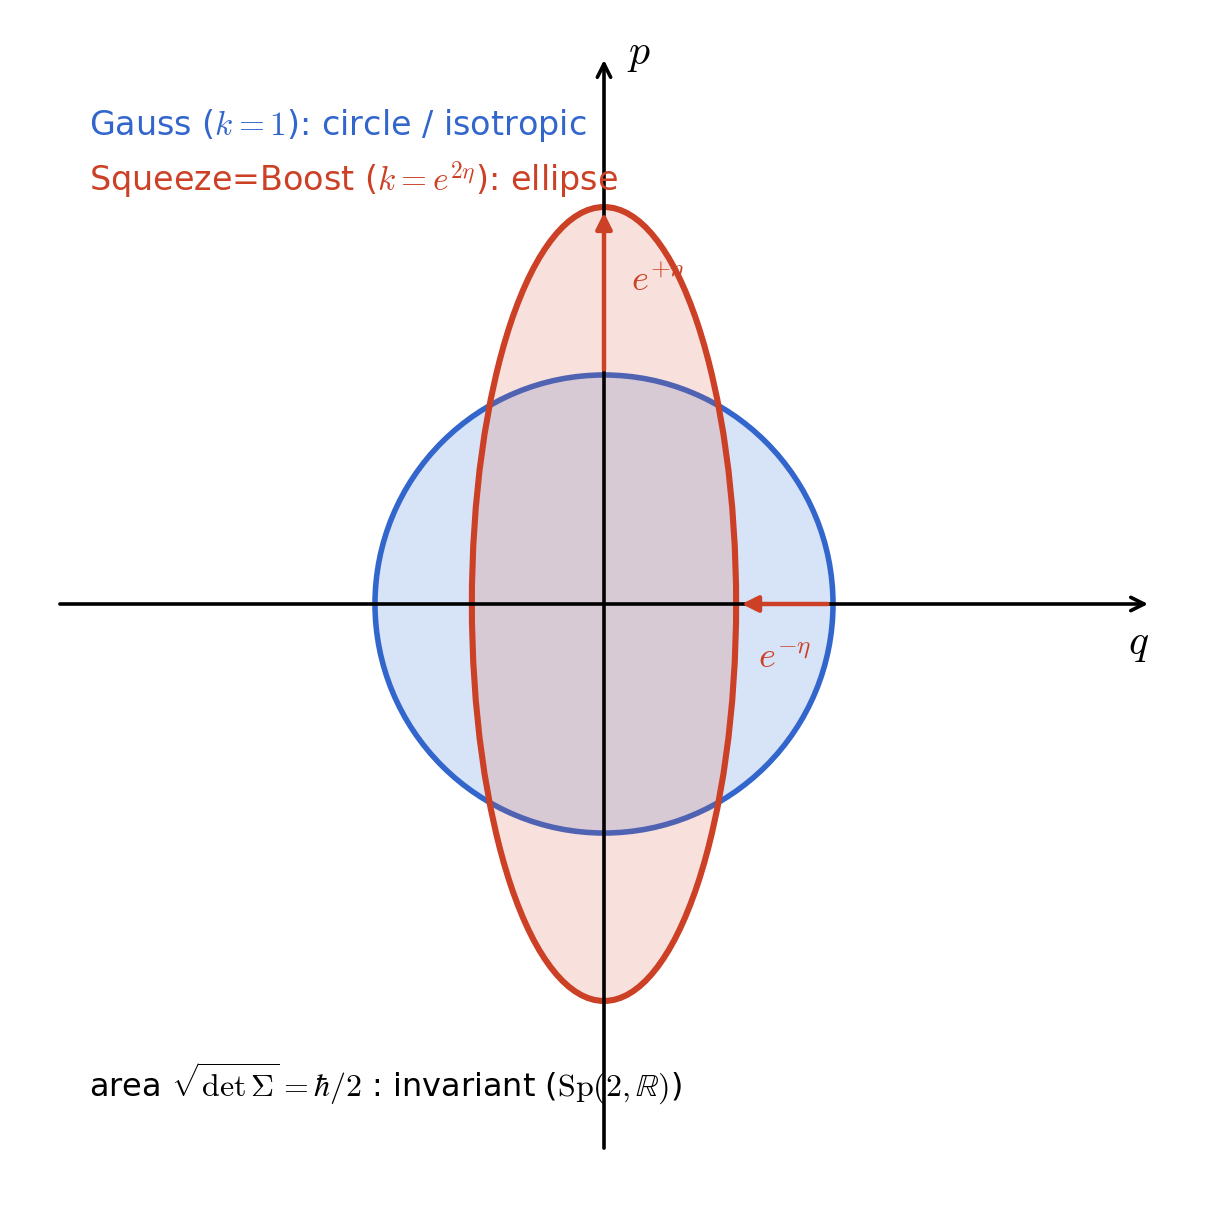
\includegraphics[keepaspectratio,alt={Fig. 1 Phase-space squeeze}]{fig1_phase_space_squeeze.png}}
\caption{Fig. 1 Phase-space squeeze}
\end{figure}

\textbf{Fig. 1}: The Gaussian ground state (blue, circle, \(k=1\),
isotropic) and a squeezed state (red, ellipse, \(k=e^{2\eta}\)) in the
phase plane \((q,p)\). The position axis is compressed by \(e^{-\eta}\)
and the momentum axis is stretched by \(e^{+\eta}\), but the symplectic
area \(\sqrt{\det\Sigma}=\hbar/2\) is invariant under the
\(\mathrm{Sp}(2,\mathbb{R})\) action. This squeeze is isomorphic to a
Lorentz boost on phase space (\(v/c=\tanh\eta\)) (§3.3).

\begin{center}\rule{0.5\linewidth}{0.5pt}\end{center}

\subsection{§4 A Generator-Theoretic Re-reading of the Imaginary Unit
and the Hyperbolic
Structure}\label{a-generator-theoretic-re-reading-of-the-imaginary-unit-and-the-hyperbolic-structure}

\subsubsection{4.1 Position of this section (preventing
misreading)}\label{position-of-this-section-preventing-misreading}

This section does \textbf{not} reject Wick rotation or standard quantum
theory. A real rotation \(e^{\theta J}\) (eigenvalues
\(e^{\pm i\theta}\) since \(J^2=-I\); compact) and a hyperbolic
evolution \(e^{\eta K}\) (eigenvalues \(e^{\pm\eta}\) since \(K^2=+I\);
non-compact) are carried into each other by the substitution
\(\theta=i\eta\). This circle\(\to\)hyperbola transition is the
\textbf{standard form of Wick rotation} (Wick 1954 {[}12{]}). Hence all
observable predictions of this section coincide with the standard
Lorentzian/Euclidean framework. What we do is confirm the formal
correspondence that Stone-type evolution and Wick-type analytic
continuation are described by the same complex structure --- not
introduce a new \(i\).

\subsubsection{4.2 Where does the complex structure come from (making
the premise
explicit)}\label{where-does-the-complex-structure-come-from-making-the-premise-explicit}

We make an important premise explicit. \textbf{Stone's theorem (Stone
1932 {[}8{]}; the uniqueness of the representation of the canonical
commutation relations is the Stone--von Neumann theorem {[}26{]})
presupposes a strongly continuous one-parameter unitary group on a
complex Hilbert space, and cannot be applied merely by projecting a real
vector space.} To speak of unitarity, the space must be equipped not
merely as a real vector space but with a complex structure (an operator
\(J\) satisfying \(J^2=-I\)). Hence this note does not claim to derive
the imaginary unit \(i\). The \(i\) is \textbf{part of a presupposed
structure} in the following sense.

The phase plane carries both the symplectic form \(\omega\) (the
\(J=\begin{pmatrix}0&1\\-1&0\end{pmatrix}\) of §3, \(=\) area) and a
positive-definite metric \(g\). When there is a positive-definite metric
compatible with the symplectic form, a \textbf{compatible almost complex
structure \(\mathcal{J}\)} satisfying

\[g(u,v)=\omega(u,\mathcal{J}v),\qquad \mathcal{J}^2=-I\]

is uniquely determined. This \(\mathcal{J}\) is the imaginary unit \(i\)
(the standard fact of Kähler structure / compatible triple, Cannas da
Silva {[}27{]}). \textbf{The \(i\) is not derived from nothing out of
real geometry; it is determined by the compatibility of two structures,
the area \(\omega\) and the metric \(g\).} This is why a complex
structure is unavoidably present in a space handling conserved
probability, and it is the structure connecting the first half of this
note (the symplectic phase plane) and the second half (the observational
projection).

\subsubsection{4.3 The form Stone's theorem assigns to the generator of
evolution}\label{the-form-stones-theorem-assigns-to-the-generator-of-evolution}

A one-parameter evolution group that preserves observation (norm =
probability preserving = unitary) can, under the complex structure of
§4.2 and by Stone's theorem, take only the form

\[U(s)=\exp(sG),\qquad G=\mathcal{J}\,H=i\,H\quad(H\ \text{self-adjoint}).\]

That is, \textbf{the quantity generating continuous evolution is
skew-adjoint (\(=i\times\) self-adjoint), and in this sense bears
\(i\).}

We correct here a common misreading. The \(i\) in
\(p=-i\hbar\,\partial_q\) is not because ``\(p\) is an unobservable
quantity'' --- momentum is an observable. This \(i\) is the
manifestation of \(p\) being the generator of spatial translation.
Likewise \(q\) generates translations in momentum space, and the two are
symmetric. \textbf{Hence \(i\) is not ``a mark intrinsic to an
unobservable axis'' but ``the representation form of the generator of
continuous evolution.''} Any self-adjoint quantity appears with \(i\) as
the generator of the corresponding one-parameter group.

\subsubsection{4.4 Re-reading the hyperbolic structure and the
identification with
Wick}\label{re-reading-the-hyperbolic-structure-and-the-identification-with-wick}

Whether the ``rotation'' of a one-parameter group acting on a
two-dimensional subspace is circular (\(\cos/\sin\), compact, Euclidean,
metric sign \(+\)) or hyperbolic (\(\cosh/\sinh\), non-compact, boost,
metric sign \(-\)) is determined by the algebraic character of its
generator --- whether it is of \(J^2=-I\) type with eigenvalues
\(\pm i\), or of \(K^2=+I\) type with eigenvalues \(\pm1\). The two are
carried into each other by the substitution \(\theta=i\eta\), isomorphic
to the Wick rotation of §4.1.

Therefore, whether a given two-dimensional plane appears as a circle
(sign \(+\)) or a hyperbola (sign \(-\)) corresponds to \textbf{whether
the observer treats the one-parameter subgroup acting on that plane as
time evolution (compact rotation) or as analytic continuation/boost
(non-compact)}. This note does \textbf{not derive} the metric signature
or the Lorentzian structure here; it is limited to \textbf{re-reading}
the hyperbolic structure already appearing in standard theory by
associating it with the algebraic character of the generator. As a
result:

\begin{itemize}
\tightlist
\item
  All observable predictions coincide with the standard
  Lorentzian/Euclidean framework.
\item
  The invariance of the speed of light \(c\) and the causal (light-cone)
  order are \textbf{inherited} because they coincide with standard SR
  (reproduced by definition, not re-derived). This is a consequence of
  this note remaining within standard theory.
\end{itemize}

\begin{figure}
\centering
\pandocbounded{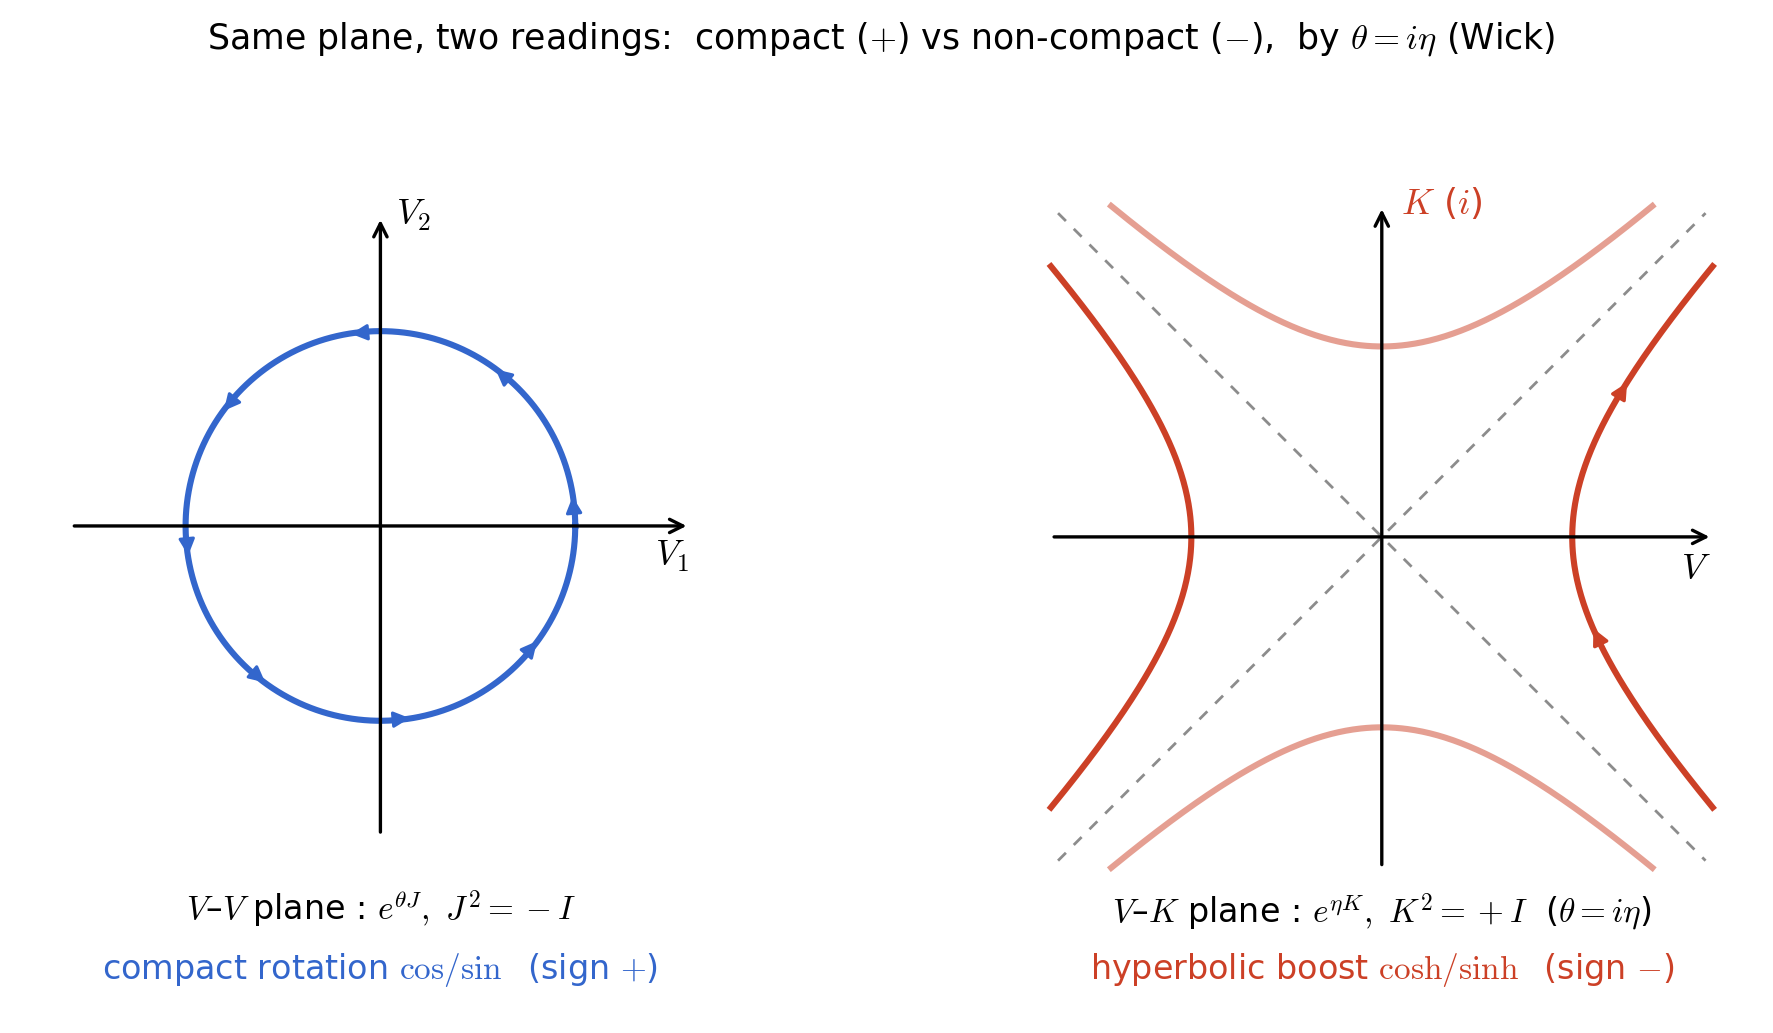
\includegraphics[keepaspectratio,alt={Fig. 2 Compact vs hyperbolic by projection}]{fig2_projection_VK.png}}
\caption{Fig. 2 Compact vs hyperbolic by projection}
\end{figure}

\textbf{Fig. 2}: One and the same two-dimensional plane splits into a
circle (\(+\)) or a hyperbola (\(-\)) according to the algebraic
character of the generator. Left: in a plane \(V\)--\(V\) within the
observable subspace, the generator is of \(J^2=-I\) type, hence compact
rotation (\(\cos/\sin\), metric sign \(+\)). Right: in a plane
\(V\)--\(K\) involving the kernel \(K\) (\(i\)-bearing evolution
generator), it is of \(K^2=+I\) type, hence a hyperbolic boost
(\(\cosh/\sinh\), metric sign \(-\)). The two are carried into each
other by the substitution \(\theta=i\eta\) (the standard form of Wick
rotation) (§4.4).

\subsubsection{\texorpdfstring{4.5 Relativity of
\(i\)}{4.5 Relativity of i}}\label{relativity-of-i}

In which direction \(i\) appears --- and hence which plane appears
hyperbolic (sign \(-\)) --- is relative to the observer's choice of
observable subspace. \textbf{This is just like how, in Wick rotation,
which coordinate direction ``imaginary time'' points to depends on the
choice of coordinates.} Taking the observable subspace in a different
orientation moves the direction treated as the evolution generator. This
relativity stays within the range observationally equivalent to standard
theory and adds no new prediction. This note is limited to this
observation.

\begin{center}\rule{0.5\linewidth}{0.5pt}\end{center}

\subsection{§5 Extension to Multiple Axes, Composite Projection, and the
Absence of Point-like
States}\label{extension-to-multiple-axes-composite-projection-and-the-absence-of-point-like-states}

\subsubsection{5.1 Observational projection and the evolution
side}\label{observational-projection-and-the-evolution-side}

In this section, the stage of projection is taken to be, as in §3--§4,
an \textbf{even-dimensional phase space} \(\mathbb{R}^{2n}\) (spanned by
\(n\) conjugate pairs \((q_i,p_i)\) and equipped with the symplectic
form \(\omega\) and the compatible almost complex structure
\(\mathcal{J}=i\) of §4.2). This is merely the natural extension of the
phase plane \((q,p)\) of §3 (a finite, boundaryless closed phase space
is already used in \(\oint p\,dq=nh\) of §2.1) and introduces no new
mechanism. Since a conjugate momentum \(p_i\) is itself a generator of
translation, the fact that a direction sent to the evolution side acts
as a generator (§4.3) is intrinsic to the structure of this phase space.

In this space, since \(\mathrm{Sp}(2n,\mathbb{R})\) acts transitively on
nonzero vectors, any axis can be chosen, \textbf{symmetrically}, as the
observable subspace \(V\) or as its complement (the kernel \(K\), the
evolution side). One may send a single axis to the kernel, or send
several axes together as a composite projection.

When a particular projection is fixed, the observable axes alone may
fail to close a developmental/dynamical description. In that case,
placing the kernel direction as an \(i\)-bearing evolution generator (by
Stone's theorem of §4, \(i\times\) self-adjoint) makes the description
consistent. In the description projected onto the observable space, this
\(i\)-bearing generator structure can be read in correspondence with the
hyperbolic structure of the plane containing that direction, or with the
metric sign \(-\) of standard theory. This note is limited to this
observation.

To forestall misreading, we state what this note does \textbf{not}
claim:

\begin{itemize}
\tightlist
\item
  It does not decide whether the causal structure is real or derivative.
\item
  \textbf{It does not claim that \(i\) is introduced because causality
  would break down.} The order is the reverse: \(i\) is an adjustment to
  make consistent a description that the observable axes alone cannot
  close, and the consistency of causality is only one aspect included in
  that consistency.
\end{itemize}

\subsubsection{5.2 Order-independence of composite
projection}\label{order-independence-of-composite-projection}

Here we add a restriction. \textbf{General projection operators do not
commute, and in the context of quantum measurement the order of
non-commuting projections is physically important.} What this note calls
``order-independence'' is a claim restricted to the \textbf{idealization
of sending mutually orthogonal independent subspaces to the evolution
side (kernel) all at once.} Under this idealization, the direct-sum
decomposition into observable/evolution sides is determined solely by
the final specification of subspaces and does not depend on which
orthogonal direction is sent first. At each step the observable
dimension decreases by \(1\) and the evolution side increases by \(1\),
but the sum

\[(\text{observable }k)+(\text{evolution side }N-k)=N\]

is preserved. The projection rule itself does not privilege a particular
axis, but once a concrete observer has chosen \(V\), the symmetry
remaining in the description is restricted to the subgroup preserving
\(V\) and \(K\) (of \(\mathrm{SO}(k)\times\mathrm{SO}(N-k)\) type). That
is, projection does not destroy the symmetry but contracts it to an
apparently lower one.

\subsubsection{5.3 On the all-evolution-side
limit}\label{on-the-all-evolution-side-limit}

Sending the observable dimension all the way to \(k=0\), all \(N\) axes
become the evolution side (formally all imaginary). In this limit, no
criterion for judging real or imaginary --- ``a mark relative to the
observable directions'' (§4.5) --- remains, so for the observer there is
no operation distinguishing all-imaginary from all-real. This is a
limiting paraphrase of the relativity of §4.5 applied at \(k=0\), not a
new claim.

Note that multiplying the whole state vector by a uniform phase is
unobservable as a global phase, but this is a different operation from
multiplying the coordinate axes / real structure by \(i\), and this note
does not identify the two.

\subsubsection{\texorpdfstring{5.4 Absence of zero-area point-like
states (a consequence of the floor
\(\tfrac12\))}{5.4 Absence of zero-area point-like states (a consequence of the floor \textbackslash tfrac12)}}\label{absence-of-zero-area-point-like-states-a-consequence-of-the-floor-tfrac12}

First, to state it precisely: what the uncertainty relation forbids is a
\textbf{zero-area quantum state} in phase space (a point-like state
satisfying \(\Delta q=\Delta p=0\)), not the origin as a mean value
\((\langle q\rangle,\langle p\rangle)=(0,0)\). The latter is taken as an
ordinary state. Hence the claim of this section is ``there is \textbf{no
zero-area point-like state} as an observable quantum state,'' not
``there is no coordinate origin.''

In this sense, \(k=0\) (all evolution side) cannot be placed as a
``definite point-like state.'' Phase space has a floor
\(\Delta q\cdot\Delta p\ge\hbar/2\) that forbids the state
\(\Delta q=\Delta p=0\). Hence ``all evolution side'' and ``total
contraction'' alike are meaningful only as \textbf{a limiting direction
that cannot close to a single point because of the floor \(\tfrac12\)},
not as a reachable point-like state.

This is consistent with the area invariance of §3. However much one
direction is compressed by squeeze (boost), the symplectic area
\(\hbar/2\) remains and does not collapse to a point-like state. The
degrees of freedom sent to the evolution side do not vanish but lie
outside observation while keeping the floor.

\begin{center}\rule{0.5\linewidth}{0.5pt}\end{center}

\subsection{§6 Relation to Existing Work, and What This Note Does Not
Claim}\label{relation-to-existing-work-and-what-this-note-does-not-claim}

\subsubsection{6.1 Relation to existing
work}\label{relation-to-existing-work}

Each component of this note is standardly established. The area
interpretation of uncertainty is Robertson 1929 {[}2{]} / Schrödinger
1930 {[}3{]}; the time--band version is Gabor 1946 {[}4{]}. The
phase-space quasi-probability distribution was discovered independently
by Wigner 1932 {[}5{]} (quantum) and Ville 1948 {[}6{]} (signal).
Sampling (Nyquist) is Shannon 1949 {[}7{]}. The relation between
one-parameter unitary groups and generators is Stone 1932 {[}8{]}. The
area-preserving transformation group and squeezed states are
\(\mathrm{Sp}(2,\mathbb{R})\) / the metaplectic representation (Folland
1989 {[}17{]}, Littlejohn 1986 {[}18{]}) and squeezed states (Stoler
1970 {[}19a{]}, Yuen 1976 {[}19{]}). The representation-theoretic origin
of \(\tfrac12\) is Bargmann 1947 {[}9{]} / Perelomov 1986 {[}10{]}. The
boundary character is the Maslov index (Maslov 1972 / Arnold 1967
{[}11{]}). This note merely re-arranges these from the common viewpoint
of area.

Regarding the interpretation of the imaginary unit \(i\) and the
hyperbolic structure, we position this note's stance against the
following. \textbf{Toward each, this note asserts no conflict, and
presents itself as an observationally equivalent re-reading.}

\begin{itemize}
\tightlist
\item
  \textbf{Wick rotation (Wick 1954 {[}12{]}) / Euclidean quantum gravity
  (Hartle--Hawking 1983 {[}13{]})}: This note reads the same
  \(\theta=i\eta\) as a formal correspondence in which the \(i\) of the
  skew-adjoint generator of Stone-type evolution and the \(i\) of
  Wick-type analytic continuation are described by the same complex
  structure. The predictions coincide.
\item
  \textbf{Relational quantum mechanics (Rovelli 1996 {[}14{]}) / QBism
  (Fuchs--Mermin--Schack 2014 {[}15{]})}: it shares the spirit of
  reading physical quantities as relations between observer and system.
\item
  \textbf{Geometric algebra (Hestenes 1966 {[}16{]})}: it reads the
  \(i\) of quantum theory as a geometric object of spacetime. This
  note's reading that ``\(i\) belongs to the generator structure''
  shares the spirit of detaching \(i\) from being an intrinsic attribute
  of coordinates, but the mechanism (the requirement of unitarity by
  Stone's theorem) differs.
\end{itemize}

\subsubsection{6.2 What this note does not
claim}\label{what-this-note-does-not-claim}

\begin{itemize}
\tightlist
\item
  Modification of the mathematical predictions of standard quantum
  theory or special relativity (this note is observationally equivalent
  to them).
\item
  Any assertion that Wick rotation or the Minkowski metric is ``wrong''
  (this is a reinterpretation, not a denial).
\item
  \textbf{Derivation of the imaginary unit \(i\), the complex structure,
  or the metric signature} (as in §4.2, \(i\) is a presupposed
  compatible almost complex structure determined by the compatibility of
  the area \(\omega\) and the metric \(g\)).
\item
  Any mention or proof of where the arrow of time comes from (this note
  does not do so, leaving it to the interpretation of existing standard
  theory).
\item
  Derivation of new physical constants, scattering cross sections, decay
  rates, or new particles.
\item
  Proof of new mathematical theorems.
\end{itemize}

\subsubsection{6.3 What this note records}\label{what-this-note-records}

\begin{itemize}
\tightlist
\item
  That the conserved quantity \(\oint p\,dq\) and the uncertainty
  \(\sqrt{\det\Sigma}\) are measured in the unit of the same symplectic
  area of the phase plane (though the numbers differ: §1.2), and that
  the half-integer structure appears in the three settings of the
  Robertson floor, the Maslov index, and the \(\mathrm{SU}(1,1)\) lowest
  weight, not as the same object but as three facets of the metaplectic
  representation.
\item
  That in the area-preserving symmetry group
  \(\mathrm{Sp}(2,\mathbb{R})\cong\mathrm{SU}(1,1)\), the Casimir is the
  representation-theoretic label of the area structure, the group action
  carries shape/allocation, and boost = non-compact subgroup = squeeze
  (\(v/c=\tanh\eta,\ k=e^{2\eta}\)).
\item
  That under the compatible almost complex structure \(\mathcal{J}=i\)
  determined by the compatibility of the area \(\omega\) and the metric
  \(g\), Stone's theorem assigns the form \(i\times\) self-adjoint to
  the generator of continuous evolution. By this, the hyperbolic
  structure of Wick rotation / Lorentz boost can be \textbf{re-read in
  the language of the observational description}, and this reading is
  observationally equivalent to standard quantum theory (not a
  derivation). Whether a given plane appears as a rotation (\(+\)) or a
  hyperbola (\(-\)) is relative to the observer's projection.
\item
  That, because of the uncertainty floor, there is no zero-area
  point-like state.
\end{itemize}

For the avoidance of doubt: \textbf{what this note means by
``identification'' is the formal correspondence that Stone-type
evolution and Wick-type analytic continuation can be described using the
same complex structure of a complex Hilbert space; it does not newly
derive Wick rotation, the Lorentzian metric, or the complex structure.}

\subsubsection{6.4 Open problems (stated explicitly as
unresolved)}\label{open-problems-stated-explicitly-as-unresolved}

The following are not treated here, or are left to a separate paper. We
state them explicitly for honesty.

\begin{enumerate}
\def\labelenumi{\arabic{enumi}.}
\tightlist
\item
  \textbf{The mechanism determining the codimension of the observable
  subspace}: which codimension an observer's projection selects
  (including the grounds for spacetime appearing as \(3+1\) in standard
  theory) is not explained within this framework (§5.1).
\item
  \textbf{Deepening the origin of the complex structure}: in §4.2, \(i\)
  was taken to be the compatible almost complex structure determined by
  the compatibility of the area \(\omega\) and the metric \(g\). To
  argue from more basic premises why this compatibility (compatible
  triple) is unavoidable for observation.
\item
  \textbf{Low-dimensional toy models and explicit forms}: to write out
  explicitly, for \(N=2,3\), the \(V\oplus K\) decomposition, the
  effective inner product, and the almost complex structure, and to
  display the form of Stone's generator \(G=iH\).
\item
  \textbf{Visualization}: the phase-plane ellipses (Gaussian vs squeezed
  state) and the boost correspondence (Fig. 1), and the schematic of the
  circle/hyperbola distinction on the \(V\)--\(V\) / \(V\)--\(K\) planes
  (Fig. 2) are included. A more detailed illustration of the multi-axis
  projection is left to future work.
\end{enumerate}

\begin{center}\rule{0.5\linewidth}{0.5pt}\end{center}

\subsection{References}\label{references}

{[}1{]} W. Heisenberg (1927). \emph{Über den anschaulichen Inhalt der
quantentheoretischen Kinematik und Mechanik}. Z. Phys. \textbf{43}, 172.
{[}2{]} H. P. Robertson (1929). \emph{The uncertainty principle}. Phys.
Rev.~\textbf{34}, 163. {[}3{]} E. Schrödinger (1930). \emph{Zum
Heisenbergschen Unschärfeprinzip}. Sitzungsber. Preuss. Akad. Wiss. 296.
{[}4{]} D. Gabor (1946). \emph{Theory of communication}. J. IEE
\textbf{93}, 429. {[}5{]} E. Wigner (1932). \emph{On the quantum
correction for thermodynamic equilibrium}. Phys. Rev.~\textbf{40}, 749.
{[}6{]} J. Ville (1948). \emph{Théorie et applications de la notion de
signal analytique}. Câbles et Transmission \textbf{2A}, 61. {[}7{]} C.
E. Shannon (1949). \emph{Communication in the presence of noise}. Proc.
IRE \textbf{37}, 10. {[}8{]} M. H. Stone (1932). \emph{On one-parameter
unitary groups in Hilbert space}. Ann. Math. \textbf{33}, 643. {[}9{]}
V. Bargmann (1947). \emph{Irreducible unitary representations of the
Lorentz group}. Ann. Math. \textbf{48}, 568. {[}10{]} A. M. Perelomov
(1986). \emph{Generalized Coherent States and Their Applications}.
Springer. {[}11{]} V. P. Maslov (1972) / V. I. Arnold (1967). \emph{On a
characteristic class entering into conditions of quantization}. Funct.
Anal. Appl. \textbf{1}, 1. {[}12{]} G. C. Wick (1954). \emph{Properties
of Bethe--Salpeter wave functions}. Phys. Rev.~\textbf{96}, 1124.
{[}13{]} J. B. Hartle, S. W. Hawking (1983). \emph{Wave function of the
Universe}. Phys. Rev.~D \textbf{28}, 2960. {[}14{]} C. Rovelli (1996).
\emph{Relational quantum mechanics}. Int. J. Theor. Phys. \textbf{35},
1637. {[}15{]} C. A. Fuchs, N. D. Mermin, R. Schack (2014). \emph{An
introduction to QBism}. Am. J. Phys. \textbf{82}, 749. {[}16{]} D.
Hestenes (1966). \emph{Space--Time Algebra}. Gordon and Breach. {[}17{]}
G. B. Folland (1989). \emph{Harmonic Analysis in Phase Space}. Princeton
Univ. Press. {[}18{]} R. G. Littlejohn (1986). \emph{The semiclassical
evolution of wave packets}. Phys. Rep.~\textbf{138}, 193. {[}19{]} H. P.
Yuen (1976). \emph{Two-photon coherent states of the radiation field}.
Phys. Rev.~A \textbf{13}, 2226. {[}19a{]} D. Stoler (1970).
\emph{Equivalence classes of minimum uncertainty packets}. Phys. Rev.~D
\textbf{1}, 3217. {[}20{]} M. de Gosson (2013). \emph{Quantum blobs}.
Found. Phys. \textbf{43}, 440. {[}21{]} D. Slepian, H. O. Pollak (1961).
\emph{Prolate spheroidal wave functions, Fourier analysis and
uncertainty I}. Bell Syst. Tech. J. \textbf{40}, 43. {[}22{]} G. H.
Hardy (1933). \emph{A theorem concerning Fourier transforms}. J. London
Math. Soc. \textbf{8}, 227. {[}23{]} R. Simon, E. C. G. Sudarshan, N.
Mukunda (1987). \emph{Gaussian--Wigner distributions in quantum
mechanics and optics}. Phys. Rev.~A \textbf{36}, 3868. {[}24{]} A. Weil
(1964). \emph{Sur certains groupes d'opérateurs unitaires}. Acta Math.
\textbf{111}, 143. {[}25{]} D. Han, Y. S. Kim, M. E. Noz (1996).
\emph{Two Different Squeeze Transformations}. arXiv:hep-th/9602019.
{[}26{]} J. von Neumann (1931). \emph{Die Eindeutigkeit der
Schrödingerschen Operatoren}. Math. Ann. \textbf{104}, 570. {[}27{]} A.
Cannas da Silva (2001). \emph{Lectures on Symplectic Geometry}.
Springer.

\begin{center}\rule{0.5\linewidth}{0.5pt}\end{center}

Author: Noriaki Kihara / WF System Co., Ltd.~/ ORCID
\href{https://orcid.org/0009-0004-6753-4020}{0009-0004-6753-4020} / CC
BY 4.0

\end{document}
